    \documentclass[tikz]{standalone}

    \usepackage{tikz}

    \begin{document}
    
    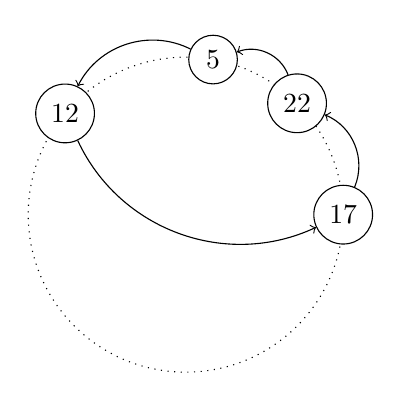
\begin{tikzpicture}
      \draw [dotted] (0,0)  circle  (2cm);
    
      \foreach \angle/\value [count = \i] in {0/17, 45/22, 80/5, 140/12} {
        \node [circle, draw, fill=white] (p\i) at (\angle:2cm) {\value}; 
        \ifnum\i=1
        \xdef\Lst{\value}
        \else
        \xdef\Lst{\Lst,\value}
        \fi
      }
      
      \foreach  [evaluate = {\j=int(mod(\i, 4)+1)}] \i in {1,...,4}  
          \draw [->] (p\i) to [bend right=45] node[midway] {\pgfkeysvalueof{/nodevalues/p\i}} (p\j) ; 
    \end{tikzpicture}


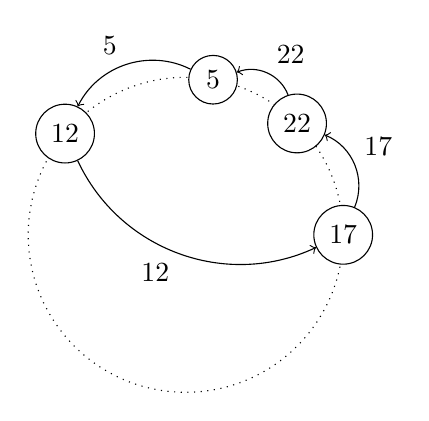
\begin{tikzpicture}
  \draw [dotted] (0,0)  circle  (2cm);
  % draw nodes on a circle, remembering their value no longer fails: 
  \foreach \angle/\value [count = \i] in {0/17, 45/22, 80/5, 140/12} {
    \node [circle, draw, fill=white] (p\i) at (\angle:2cm) {\value}; 
    \ifnum\i=1
    \xdef\Lst{\value}
    \else
    \xdef\Lst{\Lst,\value}
    \fi
  }
  % edges: 
  \foreach  [evaluate = {\j=int(mod(\i, 4)+1)}] \i in {1,...,4} 
    \pgfmathsetmacro{\X}{{\Lst}[\i-1]} 
    % \typeout{\X}
      \draw [->] (p\i) to [bend right=45] node[midway,auto,swap] 
      {\X} (p\j) ; 
\end{tikzpicture}
    
    \end{document}